\documentclass[17pt]{beamer} %Makes presentation
%\documentclass[handout]{beamer} %Makes Handouts
\usetheme{Singapore} %Gray with fade at top
\useoutertheme[subsection=false]{miniframes} %Supppress subsection in header
\useinnertheme{rectangles} %Itemize/Enumerate boxes
\usecolortheme{seagull} %Color theme
\usecolortheme{rose} %Inner color theme

\definecolor{light-gray}{gray}{0.75}
\definecolor{dark-gray}{gray}{0.55}
\setbeamercolor{item}{fg=light-gray}
\setbeamercolor{enumerate item}{fg=dark-gray}

\setbeamertemplate{navigation symbols}{}
%\setbeamertemplate{mini frames}[default]
%\setbeamercovered{dynamics}
\setbeamerfont*{title}{size=\Large,series=\bfseries}
\setbeamerfont{footnote}{size=\tiny}

%\setbeameroption{notes on second screen} %Dual-Screen Notes
%\setbeameroption{show only notes} %Notes Output

\setbeamertemplate{frametitle}{\vspace{.5em}\bfseries\insertframetitle}
\newcommand{\heading}[1]{\noindent \textbf{#1}\\ \vspace{1em}}

\usepackage{bbding,color,multirow,times,ccaption,tabularx,graphicx,verbatim,booktabs}
\usepackage{colortbl} %Table overlays
\usepackage[english]{babel}
%\usepackage[latin1]{inputenc}
%\usepackage[T1]{fontenc}
\usepackage{lmodern}

%\author[]{Thomas J. Leeper}
\institute[]{
  \inst{}%
  Department of Government\\London School of Economics and Political Science
}

\usepackage{tikz}
\usetikzlibrary{shapes,arrows,decorations.pathreplacing,calc}

\title{Sampling and Representativeness}

\date[]{}

\begin{document}

\frame{\titlepage}

\frame{\tableofcontents}

\section{Representativeness}
\frame{\tableofcontents[currentsection]}


\frame{
	\frametitle{Case selection}
	\begin{itemize}
	\item Purposive
	\item Comparative
	\item Representative
		\begin{itemize}
		\item Unrepresentative
		\end{itemize}
	\end{itemize}
}


\frame{
	\frametitle{Discuss in Pairs!}
	
	\Large
	\begin{center}
	What does it mean for a sample to be representative of a population?
	\end{center}
}

\frame{
	\frametitle{{\large Different conceptualizations\\ of representativeness}}
	
	\small
	
	\begin{itemize}\itemsep0.5em
		\item \textbf{Design-based}: A sample is representative because of how it was drawn (e.g., randomly)
		\item \textbf{Demographic-based}: A sample is representative because it resembles in the population some way (e.g., same proportion of women in sample and population, etc.)
		\item \textbf{Expert judgement}: A sample is representative as judged by an expert who deems it ``fit for purpose''
	\end{itemize}
}


\frame{
	\frametitle{Obtaining Representativeness}
	\begin{itemize}\itemsep0.5em
		\item<2-> Census
		\item<3-> Convenience/Purposive samples
		\item<4-> Quota sampling (common before 1940s)
		\item<5-> \textbf<7>{Simple random sampling}
		\item<6-> Complex survey designs
	\end{itemize}
}

\section{Model-based Selection}
\frame{\tableofcontents[currentsection]}








\section{Design-based (Statistical) Sampling}
\frame{\tableofcontents[currentsection]}

\frame{
	\frametitle{Inference from Sample to Population}
	\begin{itemize}\itemsep0.5em
	\item We want to know population parameter $\theta$
	\item We only observe sample estimate $\hat{\theta}$
	\item We have a guess but are also uncertain
	\vspace{1em}
	\item<2-> What range of values for $\theta$ does our $\hat{\theta}$ imply?
	\end{itemize}
}

\frame[label=srs]{
	\frametitle{Simple Random Sampling}
	\begin{enumerate}\itemsep0.5em
		\item Define target population
		\item Create ``sampling frame''
		\item Each unit in frame has equal probability of selection
		\item Collect data on each unit
		\item Calculate sample \textit{statistic}
		\item Draw an inference to the population
	\end{enumerate}
}


\begin{frame}[fragile]
\begin{center}
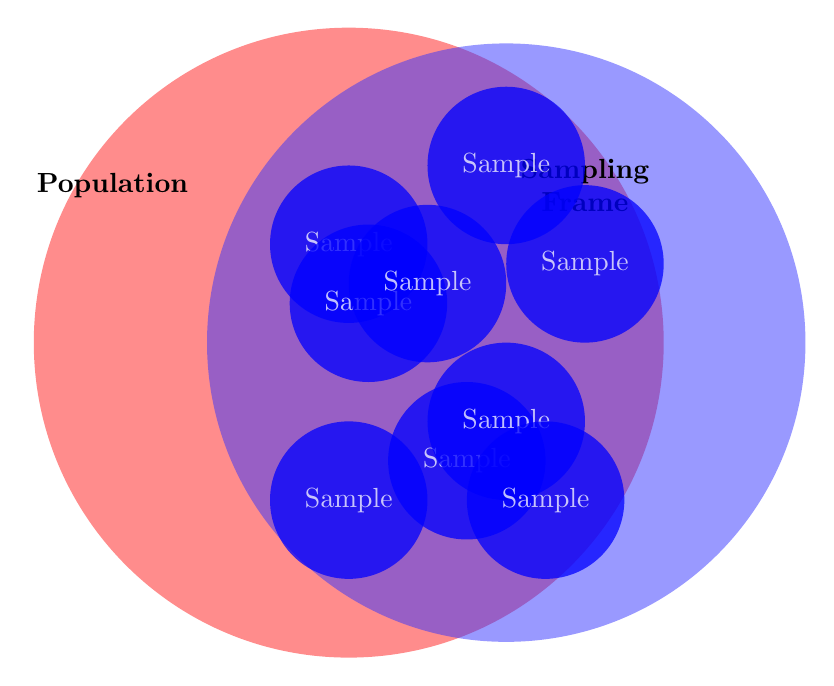
\begin{tikzpicture}
    \fill<1->[red!60,opacity=0.75] (0,0) circle (4cm) 
        node[text=white, align=center, text width=3cm] {};
    \node<1-> (pop) at (-3,2) {\textbf{Population}};
    \fill<2->[blue!80,opacity=0.5] (2,0) circle (3.8cm) 
        node[text=white, align=center, text width=3cm] {};
    \node<2->[align=center, text width=3cm] (pop) at (3,2) {\textbf{Sampling\\ Frame}};
    \fill<3->[blue,opacity=0.75] (1.5,-1.5) circle (1cm) 
        node[text=white, align=center, text width=3cm] {Sample};
    \fill<4->[blue,opacity=0.75] (3,1) circle (1cm) 
        node[text=white, align=center, text width=3cm] {Sample};
    \fill<4->[blue,opacity=0.75] (2,-1) circle (1cm) 
        node[text=white, align=center, text width=3cm] {Sample};
    \fill<4->[blue,opacity=0.75] (0,1.25) circle (1cm) 
        node[text=white, align=center, text width=3cm] {Sample};
    \fill<4->[blue,opacity=0.75] (.25,.5) circle (1cm) 
        node[text=white, align=center, text width=3cm] {Sample};
    \fill<4->[blue,opacity=0.75] (0,-2) circle (1cm) 
        node[text=white, align=center, text width=3cm] {Sample};
    \fill<4->[blue,opacity=0.75] (2,2.25) circle (1cm) 
        node[text=white, align=center, text width=3cm] {Sample};
    \fill<4->[blue,opacity=0.75] (1,.75) circle (1cm) 
        node[text=white, align=center, text width=3cm] {Sample};
    \fill<4->[blue,opacity=0.75] (2.5,-2) circle (1cm) 
        node[text=white, align=center, text width=3cm] {Sample};
\end{tikzpicture}
\end{center}
\end{frame}


\againframe{srs}

\frame{
	\frametitle{Statistical Inference I}

	To calculate a sample mean (or proportion):

	\begin{equation}
	\bar{y} = \frac{1}{n}\sum_{i=1}^{n}y_i
	\end{equation}
	{\small
	where $y_i = $ value for a unit, and\\
	$n = $ sample size
	}
	\vspace{0.5em}
	
	%This is a \textit{statistic} (the sample mean) that \textit{estimates} the population \textit{parameter} (the population mean)
	
}


\frame{
	\frametitle{Statistical Inference II}
	\begin{itemize}\itemsep1em
	\item If we calculate $\bar{y}$ in our \textit{sample}, what does this tell us about the $\bar{Y}$ in the \textit{population}?
	\item<2-> The sample \textit{estimate} is our guess at the value of the population \textit{parameter} within some degree of uncertainty
	\end{itemize}
}


\frame{
	\frametitle{Law of Large Numbers}
	\begin{itemize}
	\item Definition: The \textit{mean} of the $\hat{\theta}$ from each of a number of samples will converge on the population $\theta$, as the number of samples increases
	\end{itemize}
}

\frame{
	\frametitle{Sampling Variance}
	\begin{itemize}\itemsep1em
	\item The $\hat{\theta}$ in any particular sample can differ from the population value $\theta$
	\item This variation is calling ``sampling variance'' or ``sampling error''
	\item The standard error describes the average amount of variation of the $\hat{\theta}$'s around $\theta$
\end{itemize}
}


\frame{
	\frametitle{How Uncertain Are We?}
	\begin{itemize}\itemsep1em
	\item Our uncertainty depends on sampling procedures
	\item Most importantly, \textit{sample size}
		\begin{itemize}
		\item As $n \rightarrow \infty$, uncertainty $\rightarrow 0$
		\end{itemize}
	\item We typically summarize our uncertainty as the \textit{standard error}
	\end{itemize}
}

\frame{
	\frametitle{Standard Errors (SEs)}
	\begin{itemize}\itemsep1em
	\item Definition: ``The standard error of a sample estimate is the average distance that a sample estimate ($\hat{\theta}$) would be from the population parameter ($\theta$) if we drew many separate random samples and applied our estimator to each.''
	\item<2-> Square root of the sampling variance
\end{itemize}
}



\frame{
	\frametitle{Sample mean}
	
	\small
	
	\begin{equation}
	\bar{y} = \frac{1}{n}\sum_{i=1}^{n}y_i
	\end{equation}
	where $y_i = $ value for a unit, and\\
	$n = $ sample size
	
	\begin{equation}
	SE_{\bar{y}} = \sqrt{(1-f)\frac{s^2}{n}}
	\end{equation}
	where $f = $ proportion of population sampled,\\
	$s^2 = $ sample (element) variance, and\\
	$n = $ sample size
}

\frame{
	\frametitle{Sample proportion}
	
	\small
	
	\begin{equation}
	\bar{y} = \frac{1}{n}\sum_{i=1}^{n}y_i
	\end{equation}
	where $y_i = $ value for a unit, and\\
	$n = $ sample size
	
	\begin{equation}
	SE_{\bar{y}} = \sqrt{\frac{(1-f)}{n}p(1-p)}
	\end{equation}
	where $f = $ proportion of population sampled,\\
	$p = $ sample proportion, and\\
	$n = $ sample size
}


\frame<1>[label=moe]{

	\frametitle{Margin of Error}

	\begin{itemize}\itemsep0.5em
	\item Common to express SE as a ``margin of error''
	\item MoE is twice the Standard Error
	\item For estimated proportions, expressed as:\\
		``+/- MoE percentage points''
	\item<2-> So for an SE of 0.01, how can we describe this?
	\end{itemize}
}

\frame{
	\only<1>{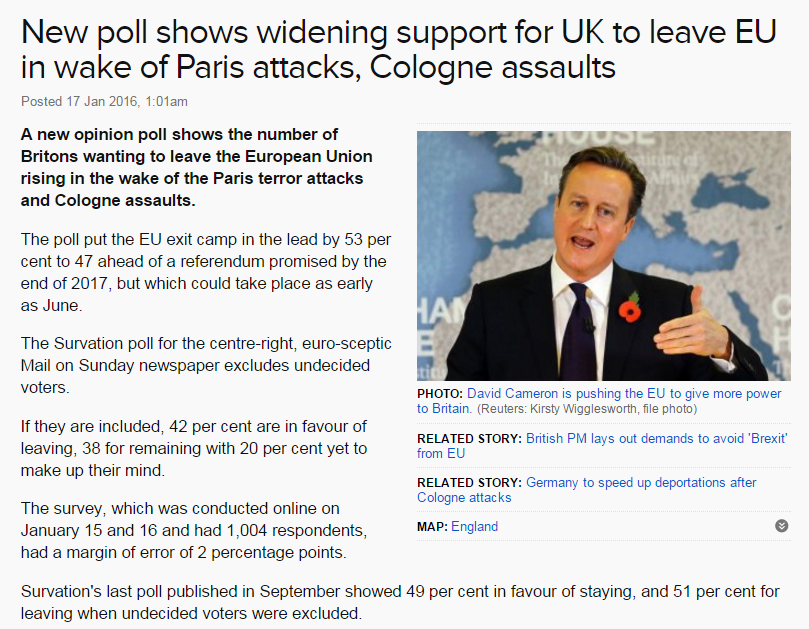
\includegraphics[height=.9\textheight]{images/ukpoll1}}
	\only<2>{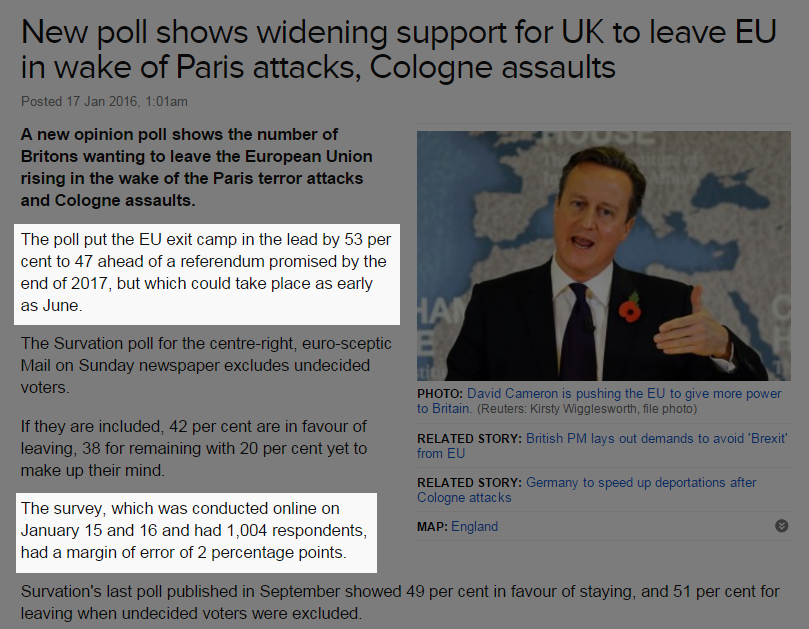
\includegraphics[height=.9\textheight]{images/ukpoll2}}
	
	{\tiny Source: \url{http://www.abc.net.au/news/2016-01-17/new-poll-show-widening-support-for-uk-to-leave-eu/7093730}\par}
}


\frame{

\LARGE

\begin{center}
Questions?
\end{center}

}

\frame{
\frametitle{Activity!}

\includegraphics[width=\textwidth]{images/haribo}

{\footnotesize Source: \href{https://www.flickr.com/people/34415916@N07}{ganeshaisis} on \href{https://commons.wikimedia.org/wiki/File:I_love_haribo_(5573044236).jpg}{Wikimedia}}

}

\frame[label=activity1]{

What proportion of all Haribo Starmix gummies are $\heartsuit$s?

	\begin{enumerate}
	\item<2-> Everyone collect a random sample
	\item<3-> Calculate $\hat{p} = \frac{\heartsuit}{n}$
	\item<4-> Report $\hat{p}$
	\item<5-> Calculate element variance: $p(1-p)$
	\item<6-> What is your margin of error?
	\end{enumerate}

}

\frame{}



\frame{
	\frametitle{{\normalsize How large of a sample do we need?}}
	\begin{itemize}\itemsep1em
	\item<2-> Uncertainty is influenced by:
		\begin{itemize}
		\item Sample size
		\item \textit{Element} variance
		\item Population size?
		\end{itemize}
	\item<3-> So what do we do?
		\begin{itemize}
		\item Decide on desired uncertainty
		\item Guess at element variance
		\item<4-> Adjust sample size based on feasibility
		\end{itemize}
	\end{itemize}
}

\frame{
	\frametitle{Estimating sample size}
    Determining sample size requires:
    	\begin{itemize}
    		\item A possible value of $p$
    		\item A desired precision (SE)
    	\end{itemize}
	\vspace{1em}
	So:
	\begin{equation}
	n = \frac{p(1-p)}{SE^2} = \frac{0.5(1-0.5)}{SE^2} = \frac{0.25}{SE^2}
	\end{equation}
	\vspace{1em}
	{\footnotesize Note: Element variance is highest when $p = 0.5$ .}
}

\frame{
	\frametitle{Estimating sample size}
	What precision (margin of error) do we want?
	\begin{itemize}\small
		\item +/- 2 percentage points: $SE = 0.01$
			\begin{equation}
			n = \frac{0.25}{0.01^2} = \frac{0.25}{0.0001} = 2500
			\end{equation}
		\item<2-> +/- 5 percentage points: $SE = 0.025$
			\begin{equation}
			n = \frac{0.25}{0.000625} = 400
			\end{equation}
		\item<3-> +/- 0.5 percentage points: $SE = 0.0025$
			\begin{equation}
			n = \frac{0.25}{0.00000625} = 40,000
			\end{equation}
	\end{itemize}
}

\frame{

	\frametitle{{\normalsize How do we reduce uncertainty?}}
	\begin{itemize}\itemsep1em
	\item<2-> Increase sample size
	\item<3-> Reduce element variance
	\item<4-> Change sampling design
		\begin{itemize}
		\item Stratified sampling\\(tends to decrease SEs)
		\item Cluster sampling\\(tends to increase SEs)
		\end{itemize}
	\end{itemize}

}




\section*{Preview}

\frame{
\frametitle{Preview}

	\begin{itemize}\itemsep1em
	\item Next week we'll discuss ethics
		\begin{itemize}
		\item Read Activity on Moodle before lecture
		\end{itemize}
	\item PS4 due December 13
	\item Sample Exam on Moodle
	\end{itemize}

}

\appendix
\frame{}

\end{document}
